\documentclass[
    left=2.5cm,
    right=2.5cm,
    top=2.5cm,
    bottom=3cm,
    bindingoffset=6mm,
    nohyphenation=false
]{szablon/eiti/eiti-thesis}

\langpol
\graphicspath{{rysunki/}}
\addbibresource{bibliografia.bib}

% Dodanie usuwa jedno z ostrzeżeń
\usepackage{csquotes}
% Dodanie tego wpływa na wyświetlanie zdjęć w odpowiedni sposób przy adnotacji [H]
\usepackage{float}
\usepackage{subfig}
\usepackage{amsmath}

\begin{document}

\DiplomaThesis
\instytut{Radioelektroniki i Technik Multimedialnych}
\kierunek{Studia Podyplomowe}
\specjalnosc{Głębokie Sieci Neuronowe - Zastosowania w Mediach Cyfrowych}
\title{
     Detekcja zalanych dróg i budynków na zdjęciach satalitarnych
}
\engtitle{
    Detection of flooded roads and buildings in satellite images
}

\author{Patryk Drobiński}
\album{P-XXXXX}

\renewcommand{\secondauthor}{Paweł Maćkowski}
\renewcommand{\secondalbum}{P-11591}

\promotor{dr Jacek Komorowski}
\date{\the\year}
\maketitle

%--------------------------------------
% Streszczenie po polsku
%--------------------------------------
\cleardoublepage % Zaczynamy od nieparzystej strony
\streszczenie

Głównym celem pracy jest
Nacisk w pracy został położony na ...
W pierwszej części pracy przedstawiono ...
Następnie opisano ...
Druga część pracy rozpoczyna się od ...
Eksperymenty opisane w dalszej części pracy przedstawiają ...
Dodatkowym etapem pracy jest ...
W zakończeniu pracy przedstawiono podsumowanie wykonanych działań
oraz dalsze działania, które mogą przynieść poprawę ...

\slowakluczowe NFT, ChatGPT, Buzzword300



% Oświadczenie o autorstwie
\cleardoublepage  % Zaczynamy od nieparzystej strony
\pagestyle{plain}
\makeauthorship

% Spis treści
\cleardoublepage % Zaczynamy od nieparzystej strony
\tableofcontents

% Rozdziały
\cleardoublepage % Zaczynamy od nieparzystej strony
\pagestyle{headings}
\newpage % Rozdziały zaczynamy od nowej strony.
\section{Wstęp}


Motywacja, dlaczego warto zająć się rozwiązaniem postawionego problemu.

Opis wkładu własnego - co zrobiono w ramach przygotowywania pracy dyplomowej. Np. przygotowanie zbioru danych, implementacja procedur to trenowania i ewaluacji modelu, opracowanie architektury modelu itp.


\newpage % Rozdziały zaczynamy od nowej strony.
\section{Cel pracy}
Niniejsza praca przedstawia rozwiązanie zadania konkursowego \textit{SpaceNet 8: Flood Detection Challenge Using Multiclass Segmentation} \cite{spacenet8}. Celem konkursu, który zakończył się w październiku 2022 roku, było wyłonienie najlepszych algorytmów wykrywających budynki i drogi, a także ich zniszczenia na skutek katastrof naturalnych, na zdjęciach satelitarnych. Oceniane były rozwiązania dwóch zagadnień:
\begin{enumerate}
\item Segmentacja budynków i dróg na pojedynczych zdjęciach oraz klasyfikacja dróg ze względu na maksymalną dozwoloną prędkość
\item Segmentacja zniszczonych budynków i dróg na podstawie par zdjęć wykonanych przed i po katastrofie naturalnej
\end{enumerate}
Ta praca skupia się na rozwiązaniu drugiego zagadnienia.
\subsection{Zbiór danych}
Zbiór danych udostępniony przez organizatorów konkursu składa się ze zdjęć satelitarnych w formacie TIFF, podzielonych na zdjęcia wykonane przed i po katastrofie, adnotacji budynków i dróg w formacie GeoJSON oraz plików CSV zawierających przypisanie adnotacji do zdjęć. Podział danych na zbiór treningowy i testowy jest zadany z góry.


\newpage % Rozdziały zaczynamy od nowej strony.
\section{Przegląd literaratury}

W \cite{vggnet} ...

W pracy \cite{unet} zaproponowano nową architekturę dla zadania semantycznej segmentacji obrazów. 


W pracy~\cite{he2016deep} opisano ....
W~\cite{liu2022convnet} zaproponowano nowatorską architekturę....
Przykładowy obraz~\ref{fig:convnext}.

\begin{figure}[h]
    \centering
    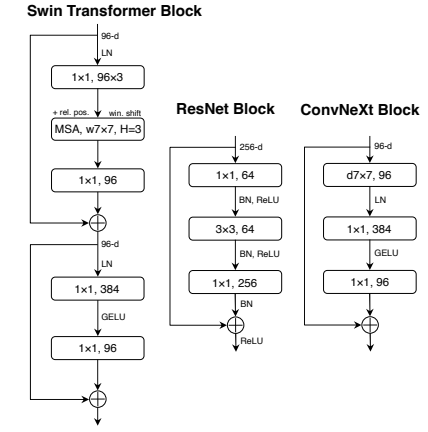
\includegraphics[width=0.5\textwidth]{rysunki/convnext_block.png}
    \caption{Porównanie bloków rezydualnych wykorzystywanych w sieci Swin Transformer, ResNet i ConvNeXt.}
    \label{fig:convnext}
\end{figure}

\newpage % Rozdziały zaczynamy od nowej strony.
\section{Opis rozwiązania}
Rozwiązanie zadania konkursowego zostało w całości zaimplementowane w języku Python w wersji 3.8. Najważniejsze biblioteki jakie zostały wykorzystane w rozwiązaniu to:
\begin{enumerate}
\item \texttt{torch} do obsługi danych i modeli.
\item \texttt{albumentations} do przetwarzania obrazów.
\item \texttt{pytorch\_lightning} do trenowania i ewaluacji modeli.
\item \texttt{segmentation-models-pytorch} do budowy modeli.
\item \texttt{neptune} do monitorowania przebiegu treningu i ewaluacji.
\end{enumerate}
\subsection{Zbiór danych}
Do wstępnej obróbki zbioru danych wykorzystano skrypty dostarczone przez organizatorów konkursu razem z rozwiązaniem \textit{baseline} w niezmienionej postaci. Przetwarzają one adnotacje w formacie GeoJSON na obrazy w formacie TIFF i rozdzielczości identycznej jak odpowiadające im zdjęcia. Dla jednej pary zdjęć (przed i po katastrofie) generowane są maksymalnie cztery obrazy:
\begin{enumerate}
\item Jednokanałowa maska budynków o wartościach $0, 1$.
\item Jednokanałowa maska dróg o wartościach $0, 1$.
\item Jednokanałowa maska dróg o wartościach 0 -- 7, odpowiadających różnym ograniczeniom prędkości. Nieużywana w tej pracy.
\item Czterokanałowa maska budynków i dróg po katastrofie o wartościach $0, 1$. Kanały odpowiadają następującym obiektom, w kolejności: niezniszczony budynek, zniszczony budynek, niezniszczona droga, zniszczona droga.
\end{enumerate}
Po przetworzeniu zbiór danych zawierał 801 par zdjęć z kompletem masek dróg i budynków przed i po katastrofie. Według podziału narzuconego w konkursie 679 par znalazło się w zbiorze treningowym i 122 w zbiorze testowym.\\
\begin{figure}[h]
\centering
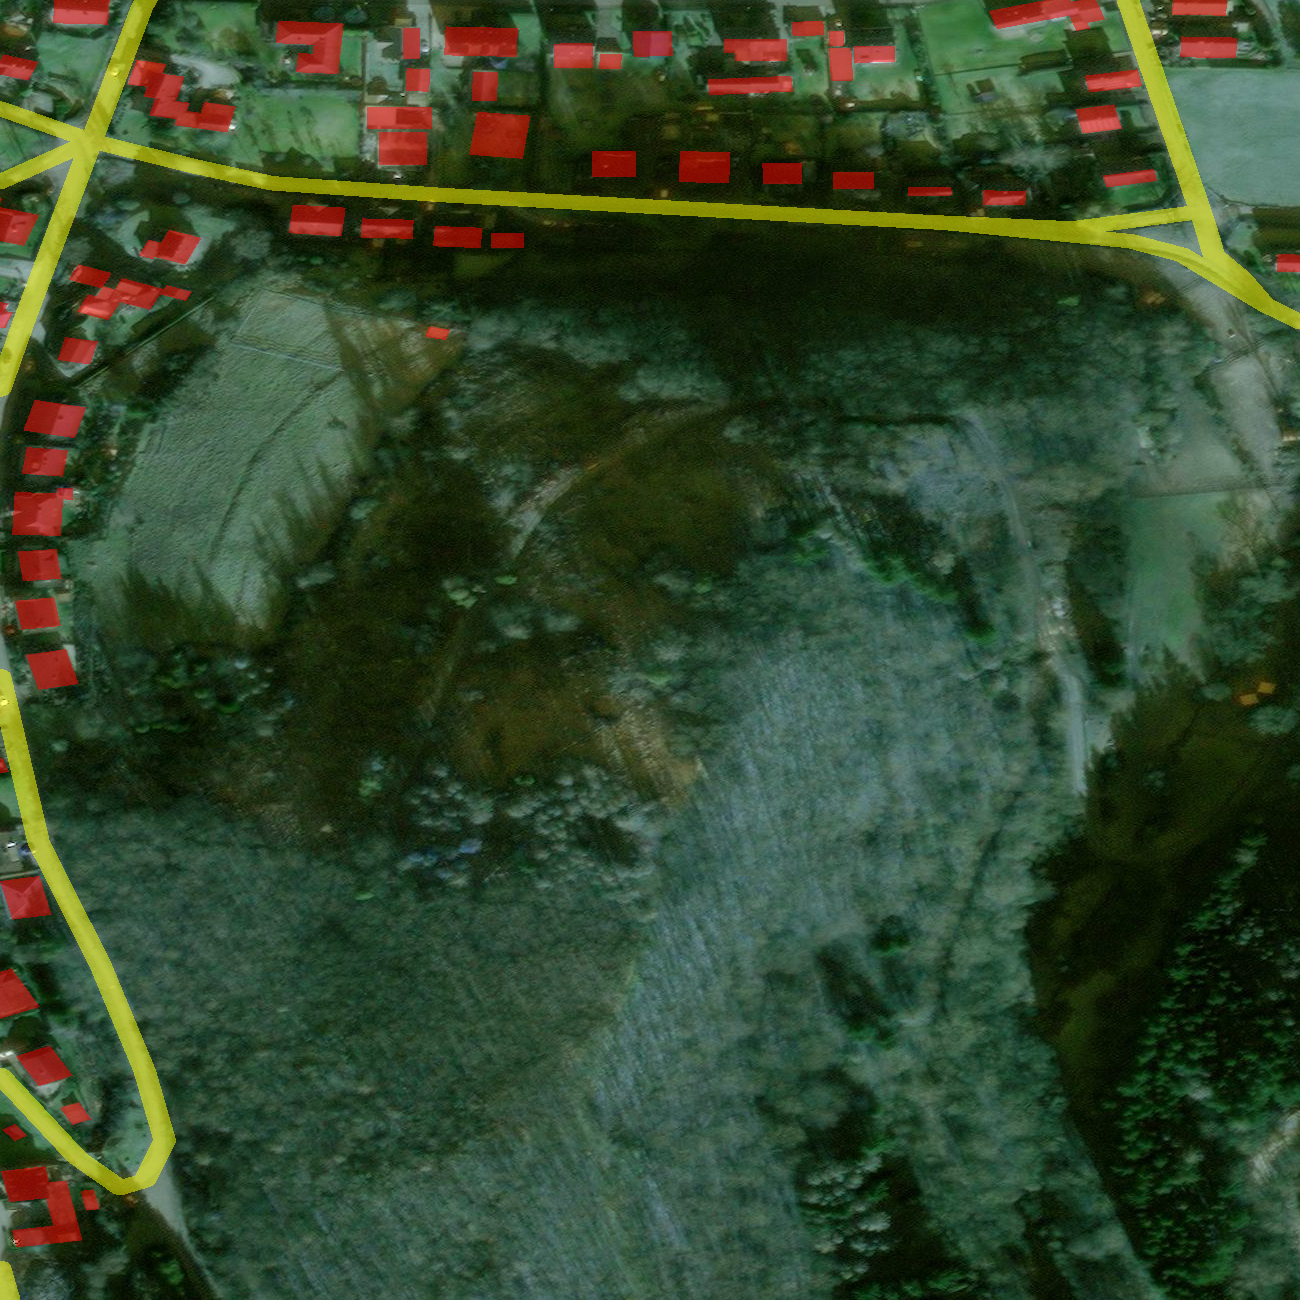
\includegraphics[width=7cm,height=7cm]{rysunki/10500500C4DD7000_0_30_69_PRE.png}
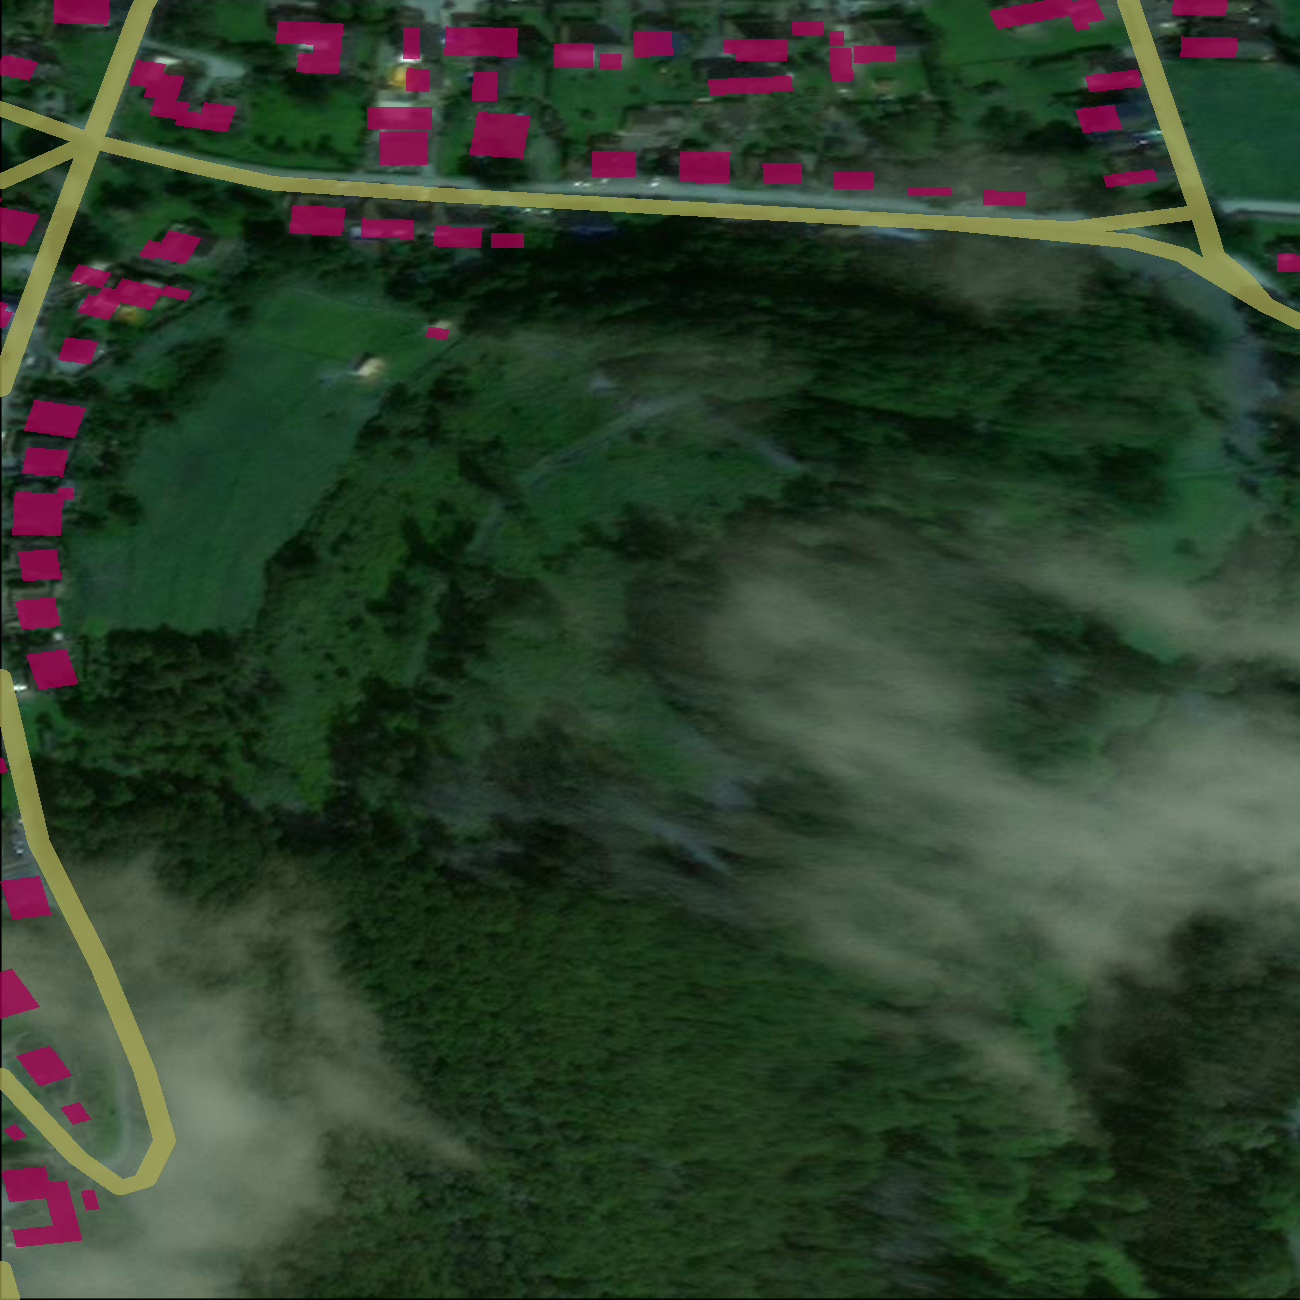
\includegraphics[width=7cm,height=7cm]{rysunki/10500500C4DD7000_0_30_69_POST.png}
\caption[Wizualizacja danych]{Przykładowa para zdjęć ze zbioru danych z adnotacjami. Wszystkie obiekty na zdjęciu po prawej są sklasyfikowane jako zniszczone.}
\end{figure}
Zdjęcia sprzed katastrofy miały rozdzielczość $1300\times 1300$ pikseli, natomiast zdjęcia po katastrofie miały różne rozdzielczości. Aby efektywnie używać ich jako wsadu do modeli o różnych architekturach, zaimplementowano skalowanie wszystkich obrazów i masek po ich wczytaniu do tej samej rozdzielczości. W eksperymentach ustalono tą rozdzielczość na $1024\times 1024$ piksele.
\subsection{Eksperymenty}


\newpage % Rozdziały zaczynamy od nowej strony.
\section{Wyniki ewaluacji eksperymentalnej}




\newpage % Rozdziały zaczynamy od nowej strony.
\section{Podsumowanie}

Podsumowanie i krytyczna analiza osiągniętych rezultatów. 
Ocena, czy osiągnięto założony cel pracy.
Dyskusja co można było zrobić lepiej i propozycja dalszych prac w celu uspraweniania opracowanego rozwiązania.


\cleardoublepage % Zaczynamy od nieparzystej strony
\printbibliography

% Spisy (opcjonalne)
\newpage
\pagestyle{plain}

\vspace{0.8cm}


\listoffigurestoc
\vspace{1cm}
\listoftablestoc

\end{document}